\chapter{Domainmodell}

\section{Architekturmodell}
Der logische Aufbau der Software besteht aus vier Schichten:
\begin{figure}[h]
	\centering
	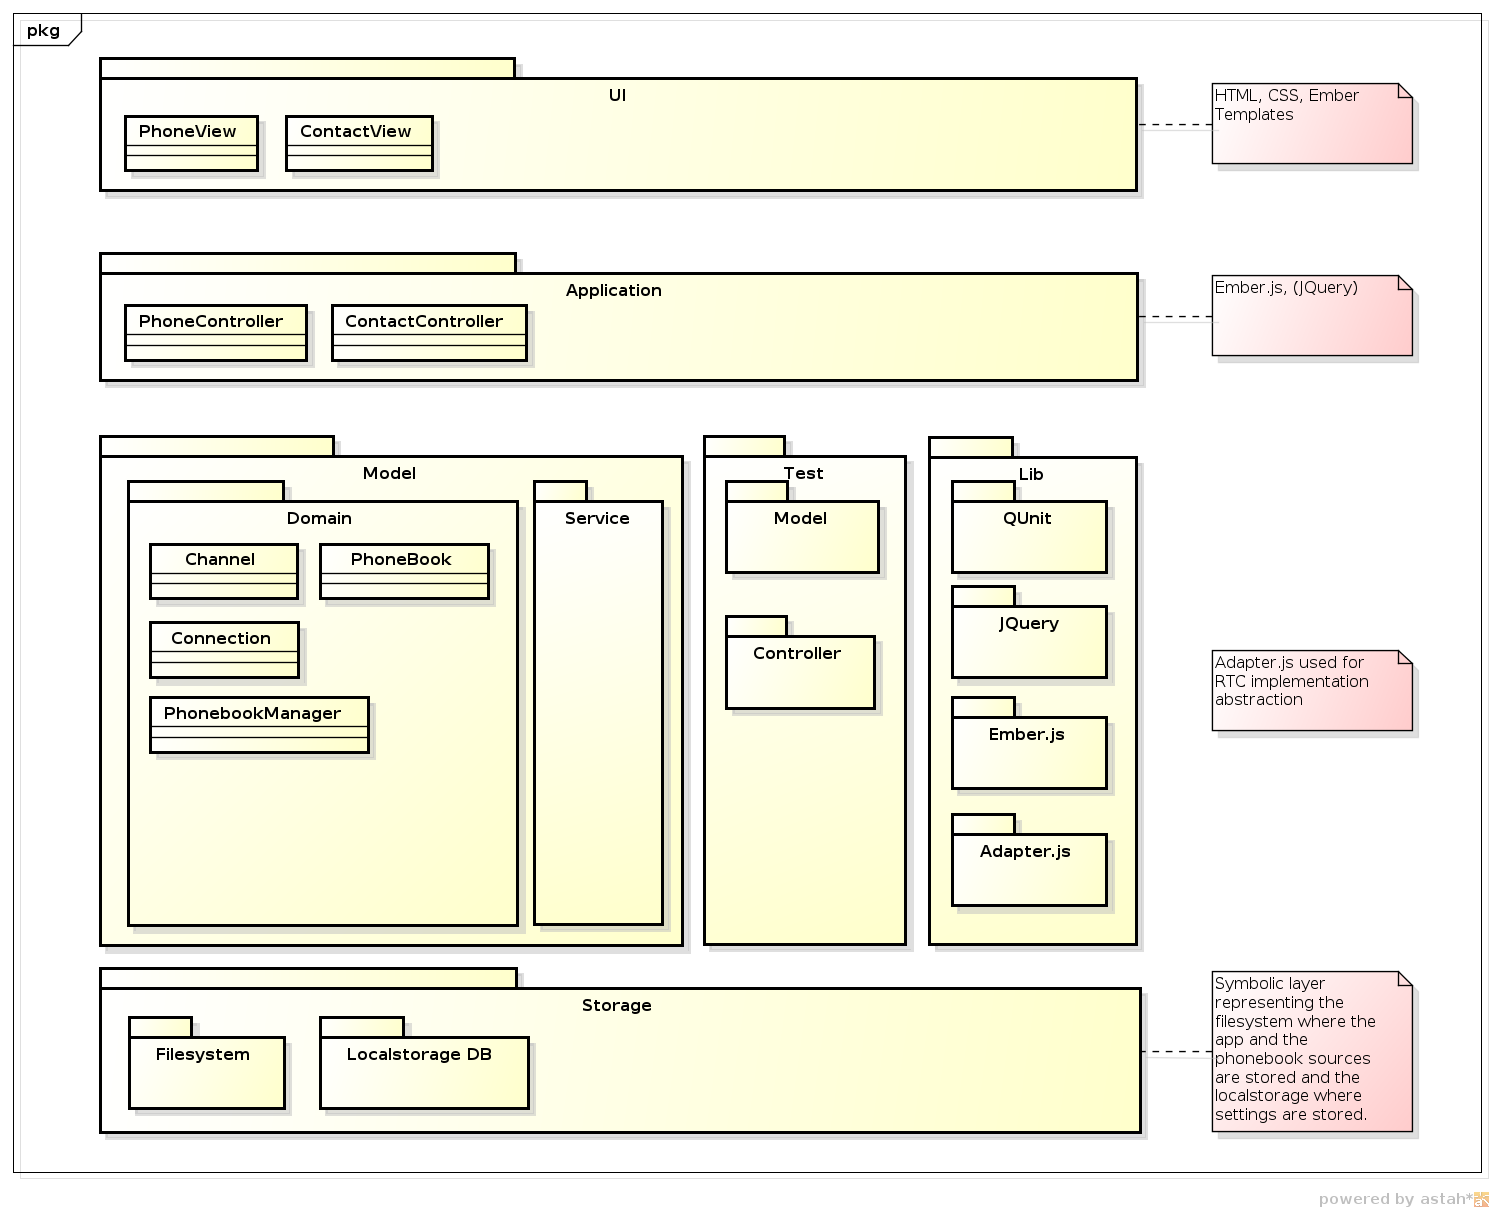
\includegraphics[width=1\textwidth]{img/architecture.png}
	\caption{Architekturdiagramm JS VoIP App}
\end{figure}

\begin{landscape}
\section{Strukturdiagramm}
Im folgenden Diagramm sind die wichtigsten konzeptionellen Klassen und ihre Beziehungen untereinander aufgeführt.
\begin{figure}[h]
	\centering
	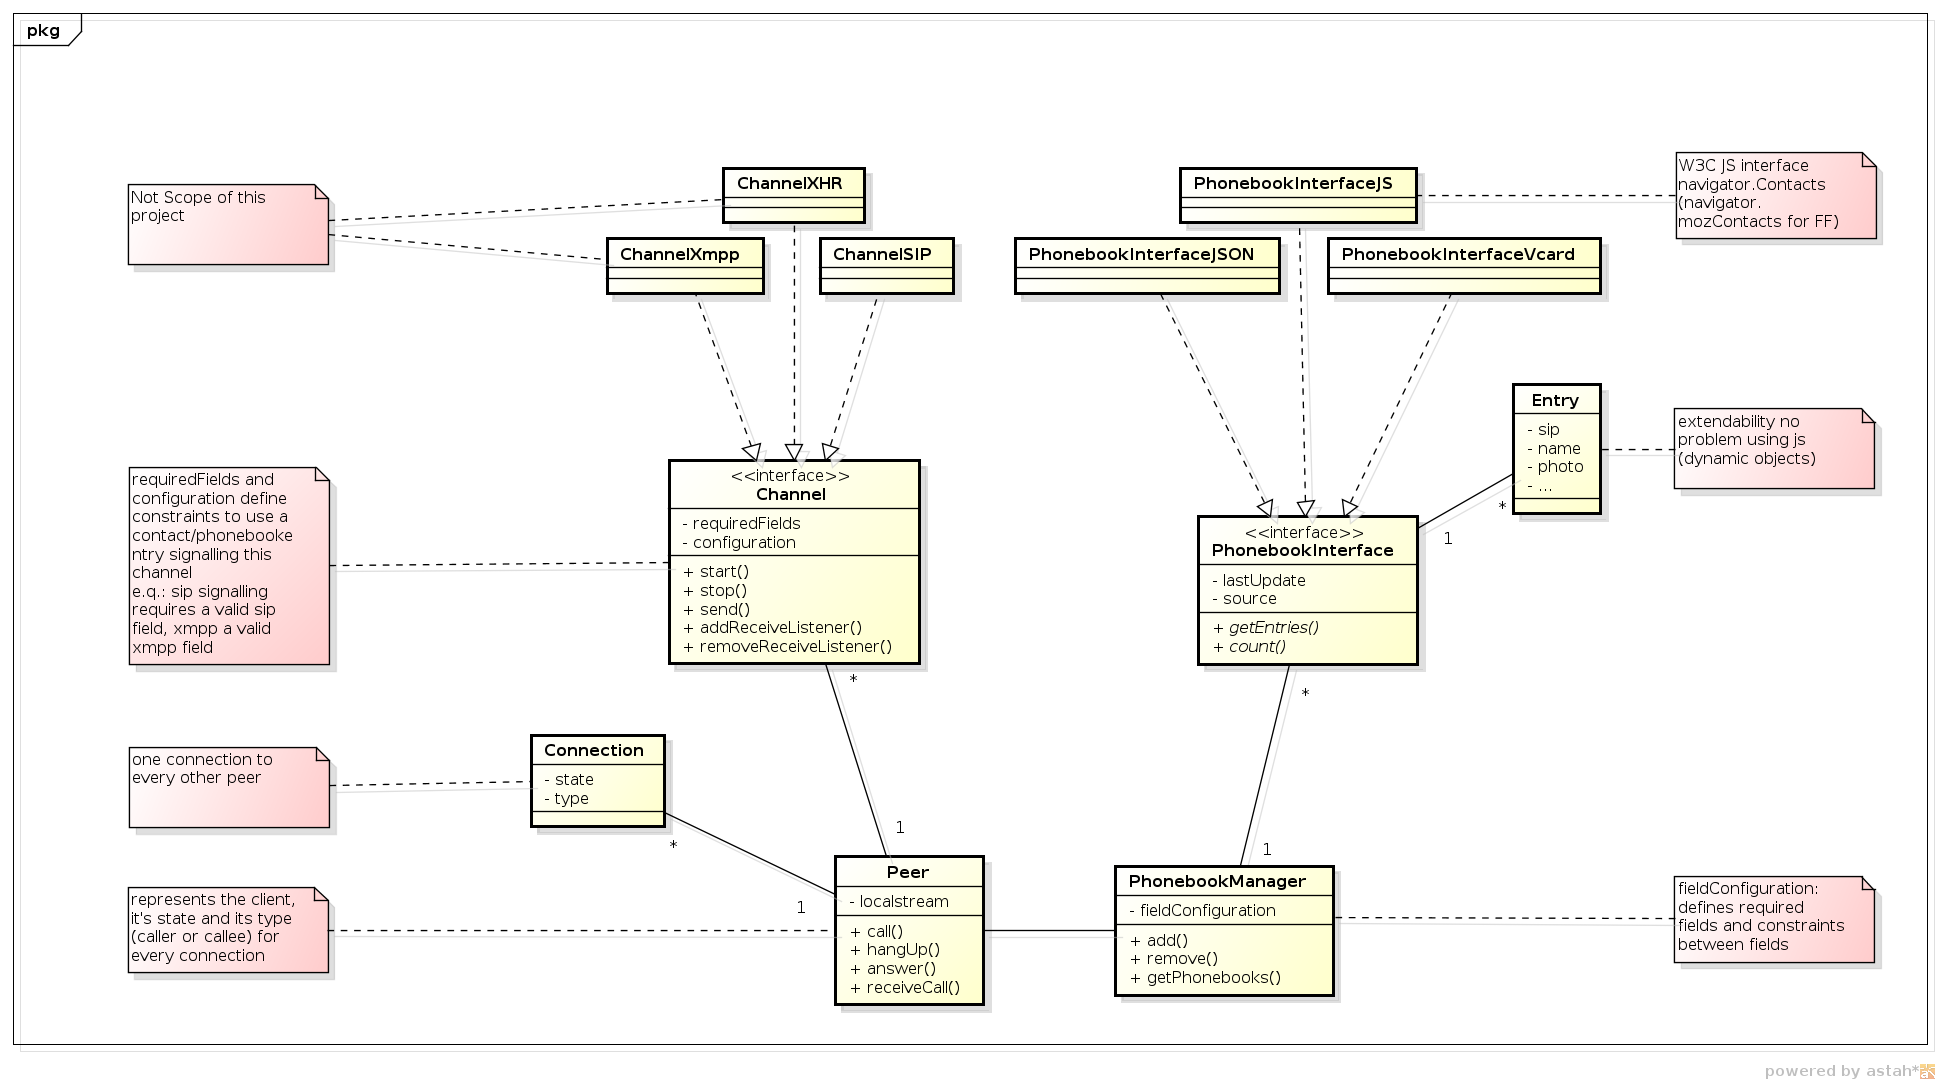
\includegraphics[width=1.2\textwidth]{img/domain.png}
	\caption{Strukturdiagramm JS VoIP App}
\end{figure}
\end{landscape}
\clearpage

\section{Deployment}
Die Applikation wird als ZIP-Datei ausgeliefert oder auf einem Webserver zur Verfügung gestellt. Der Benutzer kann die Datei entpacken und die darin enthaltene HTML Datei mit seinem Browser öffnen.
\begin{figure}[h]
	\centering
	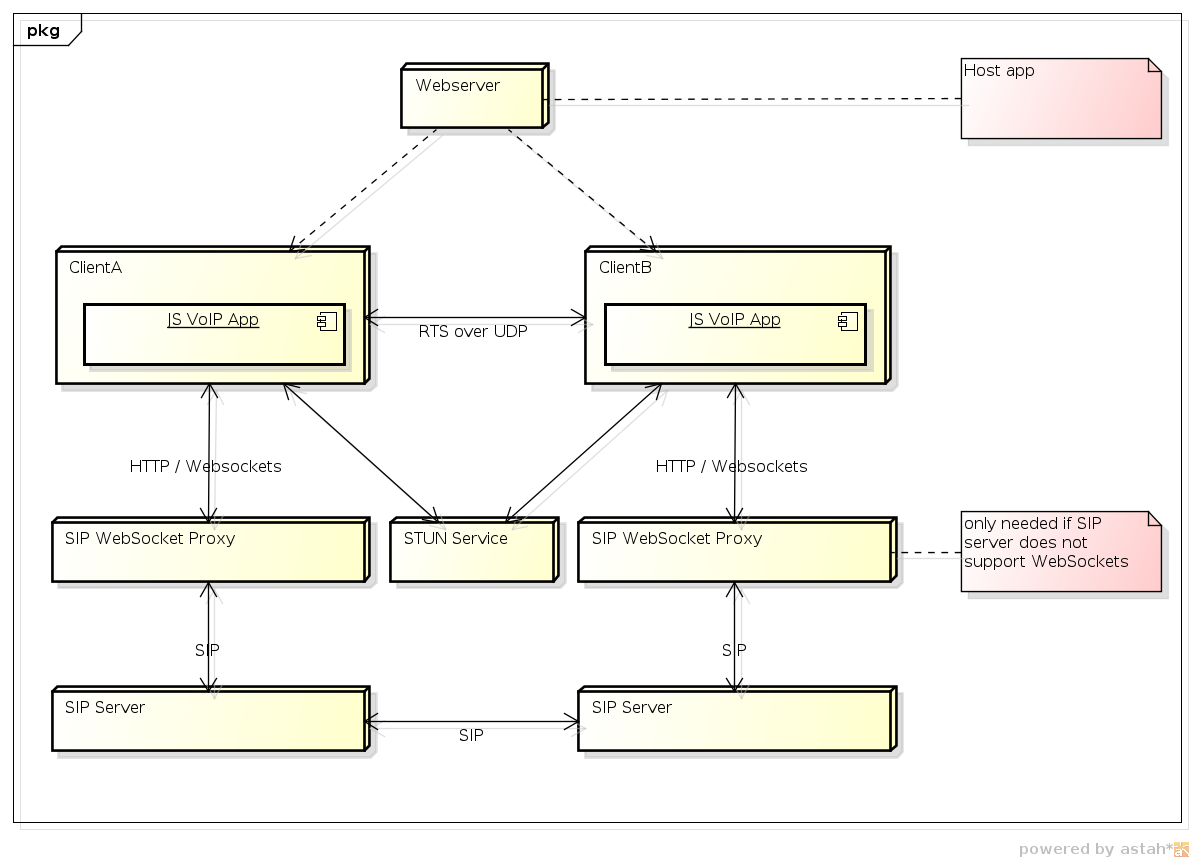
\includegraphics[width=1\textwidth]{img/deployment.png}
	\label{img:deployment}
	\caption{Deploymentdiagramm JS VoIP App}
\end{figure}
